\documentclass[xcolor=dvipsnames,t,aspectratio=169]{beamer} %t para ficar alinhado no topo do slide

\usecolortheme{rose}
\usecolortheme{dolphin}
\usetheme{Boadilla}

\usepackage[brazil]{babel} % change to brazil if needed
\usepackage[utf8]{inputenc}
\usepackage{amsfonts}
\usepackage{amsmath}
\usepackage{amssymb}
\usepackage{latexsym}
\usepackage{graphicx}
\usepackage{listings} 
\usepackage{xcolor}
\usepackage{amsthm}
\usepackage{url}
\usepackage{textpos}
\usepackage{amssymb}
\usepackage{caption}
\usepackage{subcaption}
\usepackage{multicol}
\usepackage{mathrsfs}
\usepackage{float}
\setbeamersize{text margin left=1cm,text margin right=1cm,} 
\usepackage{pythonhighlight}
\usepackage{caption}
\usepackage{subcaption}
\usepackage{dsfont}
\usepackage{physics}
\usepackage{tikz}
\usepackage{pgfplots}
% \usepackage{natbib}
\setbeamertemplate{enumerate items}[default]

\newcommand{\newauthor}[2]{
  \parbox{0.36\textwidth}{
    \texorpdfstring
      {
        \centering
        #1 \\
        {\scriptsize{\urlstyle{same}\url{#2}\urlstyle{tt}}}
      }
      {#1}
  }
}

\titlegraphic{
    
\includegraphics[scale = 0.25]{emap_logo}
}

\setlength{\parindent}{0pt} % zero indent

\setbeamertemplate{itemize items}[circle]
\setbeamertemplate{itemize subitem}{$\blacktriangleright$}

\definecolor{fgv_dark_blue}{RGB}{1, 62, 125}
\definecolor{fgv_light_blue}{RGB}{6, 143, 203}
\setbeamercolor{normal text}{fg=fgv_dark_blue}\usebeamercolor*{normal text}
\setbeamercolor{math text}{fg=fgv_light_blue}\usebeamercolor[fg]{math text}

\setbeamercolor{title}{fg=fgv_dark_blue}
\setbeamercolor{frametitle}{fg=fgv_dark_blue}
\setbeamercolor{structure}{fg=fgv_dark_blue}
\setbeamercolor{author}{fg=fgv_light_blue}
\setbeamercolor{footline}{fg=fgv_dark_blue} 

\setbeamertemplate{footline}[frame number]
\setbeamertemplate{navigation symbols}{}

\definecolor{codegreen}{rgb}{0,0.6,0.2}
\definecolor{codegray}{rgb}{0.5,0.5,0.5}
\definecolor{codepurple}{rgb}{0.58,0,0.82}
\definecolor{backcolour}{rgb}{0.95,0.95,0.92}

\lstdefinestyle{mystyle}{
    backgroundcolor=\color{backcolour},   
    commentstyle=\color{codegreen},
    keywordstyle=\color{magenta},
    numberstyle=\tiny\color{codegray},
    stringstyle=\color{codepurple},
    basicstyle=\ttfamily\footnotesize,
    breakatwhitespace=false,  
    breaklines=true,                 
    captionpos=b,                    
    keepspaces=true,                 
    numbers=left,                    
    numbersep=5pt,                  
    showspaces=false,                
    showstringspaces=false,
    showtabs=false,                  
    tabsize=2
}

\lstset{style=mystyle}

\newcommand{\highlight}[1]{{\color{fgv_light_blue} #1}}

\newcommand{\ds}{\displaystyle}
\newcommand{\nl}{\newline}
\newcommand{\eps}{\varepsilon}
\newcommand{\ssty}{\scriptstyle}
\newcommand{\bE}{\mathds{E}}
\newcommand{\cB}{\mathcal{B}}
\newcommand{\cF}{\mathcal{F}}
\newcommand{\cA}{\mathcal{A}}
\newcommand{\cM}{\mathcal{M}}
\newcommand{\cD}{\mathcal{D}}
\newcommand{\cP}{\mathcal{P}}
\newcommand{\cN}{\mathcal{N}}
\newcommand{\cL}{\mathcal{L}}
\newcommand{\cLN}{\mathcal{LN}}
\newcommand{\bP}{{\rm I\!P}}
\newcommand{\bQ}{\mathbb{Q}}
\newcommand{\bN}{{\rm I\!N}}
\newcommand{\bR}{\mathds{R}}
\newcommand{\bZ}{\mathbb{Z}}
\newcommand{\bC}{\mathbb{C}}
\newcommand{\ind}{\mathds{1}}
\newcommand{\data}{\mathcal{D}}
\newcommand{\bV}{\mathds{V}}

% \renewcommand{\boldsymbol}{\symbf}

\newcommand{\bfP}{\boldsymbol{P}}
\newcommand{\bfQ}{\boldsymbol{Q}}
\newcommand{\bfX}{\boldsymbol{X}}
\newcommand{\bfY}{\boldsymbol{Y}}
\newcommand{\bfZ}{\boldsymbol{Z}}
\newcommand{\bfM}{\boldsymbol{M}}
\newcommand{\bfU}{\boldsymbol{U}}

\newcommand{\bfz}{\boldsymbol{z}}
\newcommand{\bfm}{\boldsymbol{m}}
\newcommand{\bfw}{\boldsymbol{w}}
\newcommand{\bfv}{\boldsymbol{v}}
\newcommand{\bfu}{\boldsymbol{u}}
\newcommand{\bfx}{\boldsymbol{x}}
\newcommand{\bfy}{\boldsymbol{y}}
\newcommand{\bfb}{\boldsymbol{b}}
\newcommand{\bfa}{\boldsymbol{a}}
\newcommand{\bfp}{\boldsymbol{p}}
\newcommand{\bff}{\boldsymbol{f}}
\newcommand{\tbx}{\tilde{\bfx}}
\newcommand{\tby}{\tilde{\bfy}}
\newcommand{\tbf}{\tilde{\bff}}
\newcommand{\yst}{\boldsymbol{y_\star}}
\newcommand{\fst}{\boldsymbol{f_\star}}
\newcommand{\xst}{\boldsymbol{x_\star}}
\newcommand{\bfth}{\boldsymbol{\theta}}
\newcommand{\bfmu}{\boldsymbol{\mu}}
\newcommand{\bfxi}{\boldsymbol{\xi}}
\newcommand{\bfsg}{\boldsymbol{\sigma}}


\newcommand{\htheta}{\hat{\theta}}
\newcommand{\poi}{\text{Poisson}}
% \newcommand{\var}{\text{Var}}
\newcommand{\cov}{\text{Cov}}
\newcommand{\gama}{\text{Gama}}
\newcommand{\normal}{\text{Normal}}
\newcommand{\ig}{\text{Inverse-Gamma}}
\newcommand{\ber}{\text{Bernoulli}}
\newcommand{\jg}{\text{Jg}}
\newcommand{\st}{\text{ s.t. }}
\newcommand{\otw}{\text{ otherwise }}
\newcommand{\sge}{\sigma_e^2}
\newcommand{\sgt}{\sigma_\theta^2}
\newcommand{\byi}{\bar{y}_i}
\newcommand{\gp}{\mathcal{GP}}

\newcommand{\dU}{\mathcal{U}}

\title{Eigenfaces: \\ Uma Análise Comparativa entre PCA e SVD} %Published by {\color{fgv_light_blue} Stef van den Elzen} and {\color{fgv_light_blue}Jarke J. van Wijk} @ Eindhoven University of Technology}
\author{
\newauthor{Beatriz Miranda}{beatriz.bezerra@fgv.edu.br}
\and
\newauthor{Gustavo Murilo}{gustavo.carvalho.2023@fgv.edu.br}
}

\date{{\color{fgv_dark_blue}  \textbf{Rio de Janeiro, Brasil}\\ \today}}

\begin{document}

\frame[plain]{\titlepage}

\logo{
\begin{tikzpicture}[overlay,remember picture]
\node[left=1.1cm, below=0.2cm] at (current page.30){
    
\includegraphics[width=0.165\textwidth]{emap_logo}};
\end{tikzpicture}
}

\begin{frame}[c]{Introdução}
\framesubtitle{Uma possível aplicação das Eigenfaces}


    \begin{block}{Rosto médio de mulheres de diferentes países}

        \begin{figure}[H]
                  \centering
                  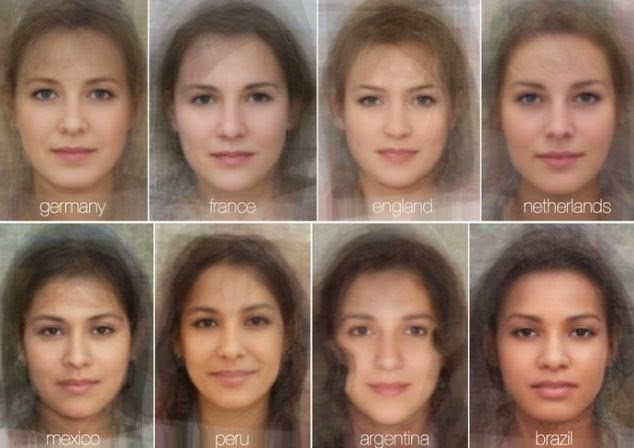
\includegraphics[width=0.5\textwidth]{img/rostomedio.jpg}
                 %\caption{}
                  \label{fig:exemplo}
            \end{figure}
    
    \end{block}

\end{frame}

\begin{frame}[c]{SVD e PCA}

    \begin{block}{Resumidamente, as etapas para aplicação do PCA são:}
    
        \begin{enumerate}
            \item Escolher variáveis (dimensões) a serem avaliadas;
            \item Subtrair média de cada dimensão, produzindo um conjunto de dados com média zero;
            \item Calcular matriz de covariância;
            \item Calcular os autovetores e autovalores da matriz de covariância;
            \item Escolher as $k$ componentes principais ($k$ autovetores com maior autovalor)
            \item Interpretar as informações contidas nas componentes principais.
        \end{enumerate}
                    
    \end{block}

\end{frame}

\begin{frame}[c]{SVD e PCA}
    
        \begin{block}{A Principal diferença entre PCA e SVD}
        \begin{itemize}
            \item No entanto, é possível substituir a etapa $4$ pela aplicação do SVD, uma vez que os $k$ primeiros autovetores da matriz de covariância são as $k$ dimensões de maior variabilidade. Neste sentido, podemos interpretar o PCA como o processo de fatoração do SVD, aplicado à matriz de covariância.
            \begin{itemize}
                \item Assim, salvo as devidas diferenças teóricas, a questão prática se reduz à identificarmos as diferenças entre SVD sobre a matriz de covariância e SVD sobre a matriz original.
            \end{itemize}
        \end{itemize}
    
\end{block}

\end{frame}

\begin{frame}[c]{Eigenfaces}
\framesubtitle{Calculo da face média}

     Definimos então a $i$-ésima imagem como $\boldsymbol{a_i} \in \mathds{R}^{mn}$ tal que $1 \leq i \leq q$, onde $q$ é o número de imagens no banco de dados. A partir delas, é criada a matriz que contém todas as imagens originais, $\boldsymbol{A} \in \mathds{R}^{mn \times q}$.
        
            $$
            \boldsymbol{A} = \begin{bmatrix} \boldsymbol{a_1} & \boldsymbol{a_1} & \ldots & \boldsymbol{a_q} \end{bmatrix}
            $$
    Face média:
            $$
            \boldsymbol{f_\mu} = \frac{1}{q} \sum_{i=1}^{q} \boldsymbol{a_i}
            $$

\end{frame}




            
\begin{frame}[c]{Eigenfaces}
\framesubtitle{Face média}

        \hfill
        \begin{figure}[H]
              \begin{subfigure}{0.4\textwidth}
                \centering
                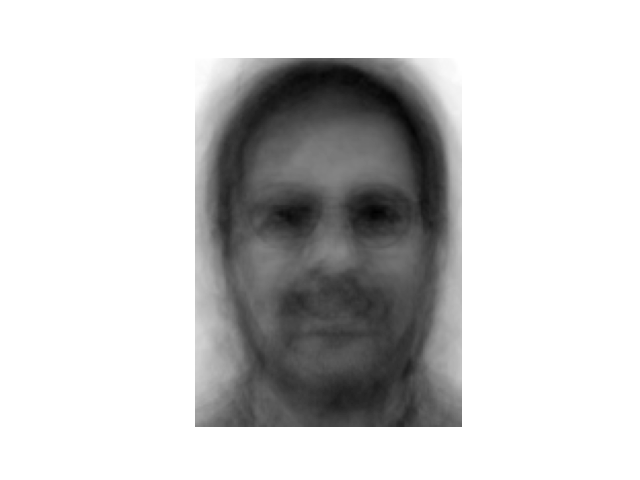
\includegraphics[width=\textwidth]{img/EMAP_0.png}
                \caption{Corpo docente da EMAp.}
                \label{fig:imagem1}
              \end{subfigure}
              \hfill
              \begin{subfigure}{0.4\textwidth}
                \centering
                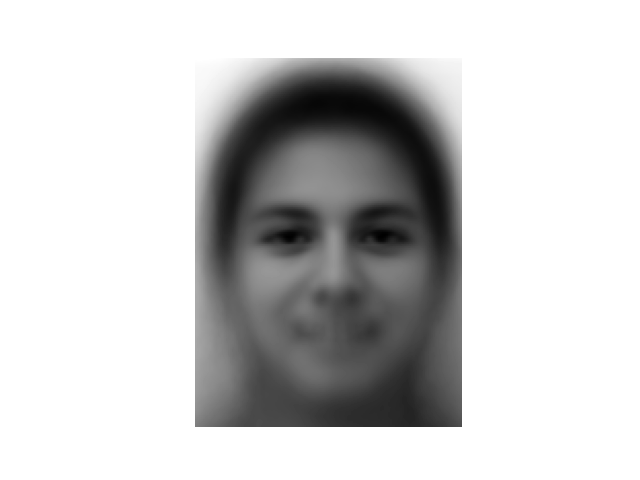
\includegraphics[width=\textwidth]{img/MAIN_0.png}
                \caption{FEI Face Database.}
                \label{fig:imagem2}
              \end{subfigure}
              \caption{Face média}
            \end{figure}
              \hfill

\end{frame}

\begin{frame}[c]{Eigenfaces}
\framesubtitle{Cálculo da matriz de covariância}
     Em seguida, definimos a matriz com os dados centralizados $\boldsymbol{M}$ por:

            $$
            \boldsymbol{m_i} = \sum_{i=1}^{q} \boldsymbol{a_i} - \boldsymbol{f_\mu}
            $$        

            $$
            \boldsymbol{M} = \begin{bmatrix}
            \mid & \mid & \ldots  & \mid \\
            \boldsymbol{m_1} & \boldsymbol{m_2} & \ldots & \boldsymbol{m_q}\\
            \mid & \mid & \ldots  & \mid
            \end{bmatrix}
            $$

            
           A matriz de covariância amostral do nosso conjunto de dados, denotada por $\boldsymbol{C} \in  \mathds{R}^{mn \times mn}$ pode ser calculada da seguinte maneira:

            $$
            \boldsymbol{C} = \frac{1}{q-1} \sum_{i=1}^{q} (\boldsymbol{a}_i - \boldsymbol{f_\mu}) (\boldsymbol{a}_i - \boldsymbol{f_\mu})^T = \frac{1}{q-1} \boldsymbol{M} \boldsymbol{M}^T
            $$
    
\end{frame}

\begin{frame}[c]{Eigenfaces}
\framesubtitle{Correção pela média}

        \begin{figure}[H]
                  \centering
                  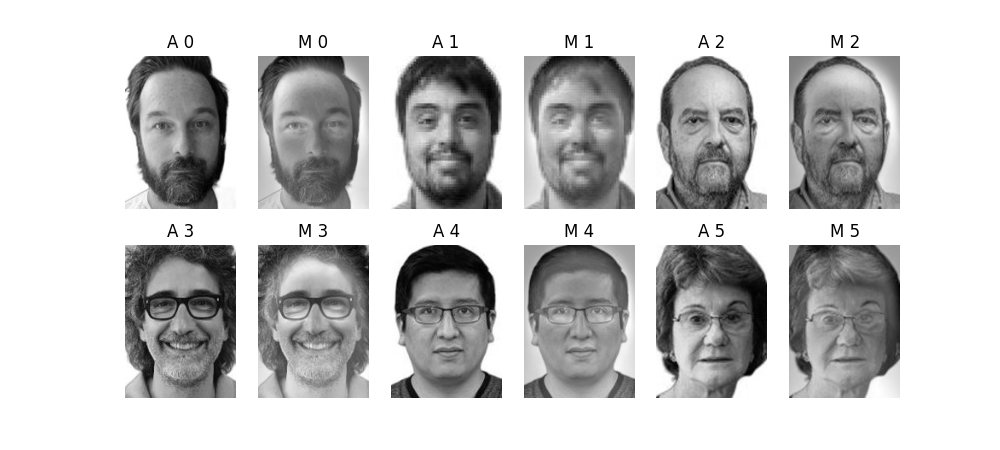
\includegraphics[width=1\textwidth]{img/MAIN_1.png}
                  \caption{Imagens corrigidas pela média}
                  \label{fig:exemplo}
            \end{figure}

\end{frame}

\begin{frame}[c]{Eigenfaces}
\framesubtitle{Aplicação do PCA}
     Observe que $\boldsymbol{C}$ é simétrica e positiva definida, portanto, aplica-se o teorema espectral. A decomposição da matriz de covariância $\boldsymbol{C}$ usando a SVD é dada por:

            $$
            \boldsymbol{C} = \boldsymbol{U} \boldsymbol{\Sigma} \boldsymbol{V}^{T}  = \boldsymbol{U} \boldsymbol{\Sigma} \boldsymbol{U}^{T}
            $$

     onde $\boldsymbol{U}$ é a matriz de autovetores e $\boldsymbol{\Sigma}$ é uma matriz diagonal contendo os autovalores em ordem decrescente. Os autovetores em $\boldsymbol{U}$ são chamados de "eigenfaces". Eles representam as principais componentes de variação nas imagens faciais.
    
\end{frame}

\begin{frame}[c]{Eigenfaces}
\framesubtitle{Eigenfaces mais relevantes}

        \begin{figure}[H]
                  \centering
                  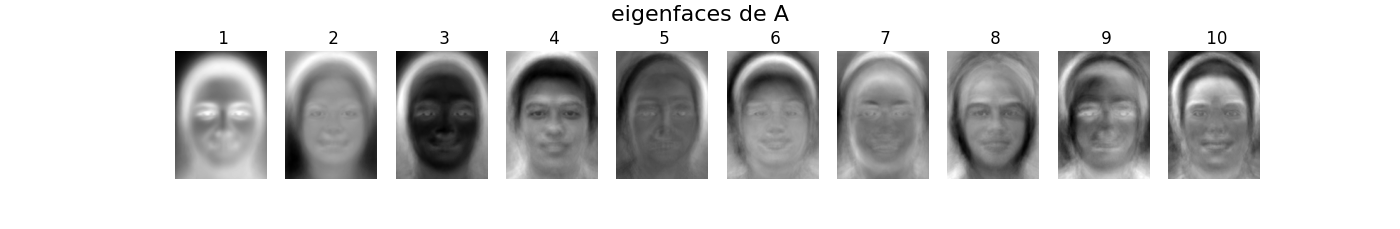
\includegraphics[width=1\textwidth]{img/MAIN_2.png}
                  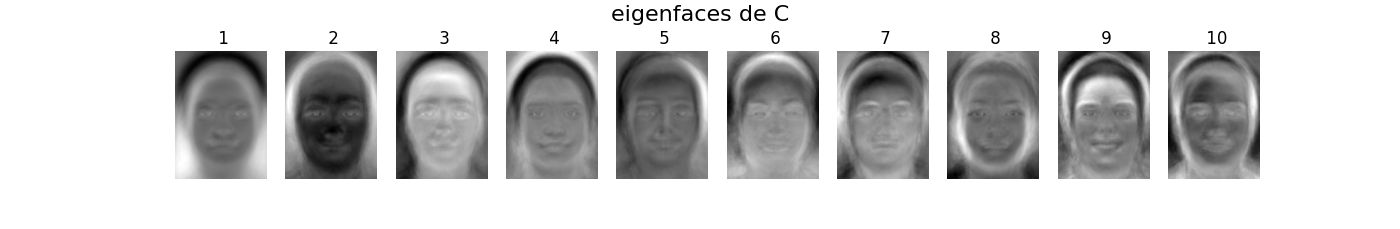
\includegraphics[width=1\textwidth]{img/MAIN_3.png}
                  \caption{Eigenfaces mais relevantes de cada matriz}
                  \label{fig:exemplo}
            \end{figure}

\end{frame}

\begin{frame}[c]{Eigenfaces}
\framesubtitle{Eigenfaces menos relevantes}

        \begin{figure}[H]
                  \centering
                  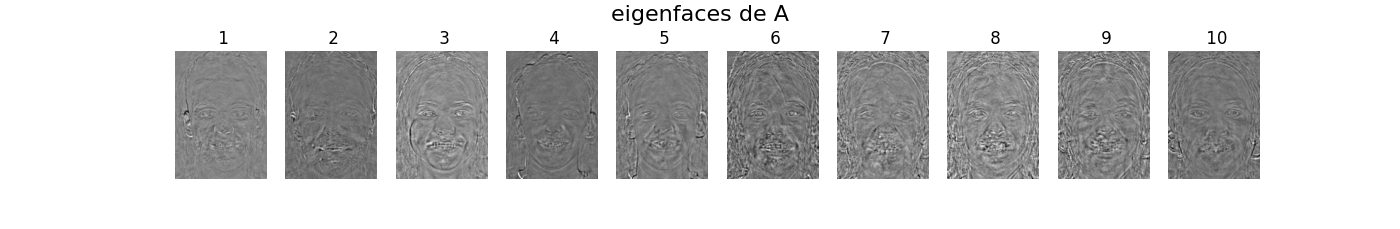
\includegraphics[width=1\textwidth]{img/MAIN_4.png}
                  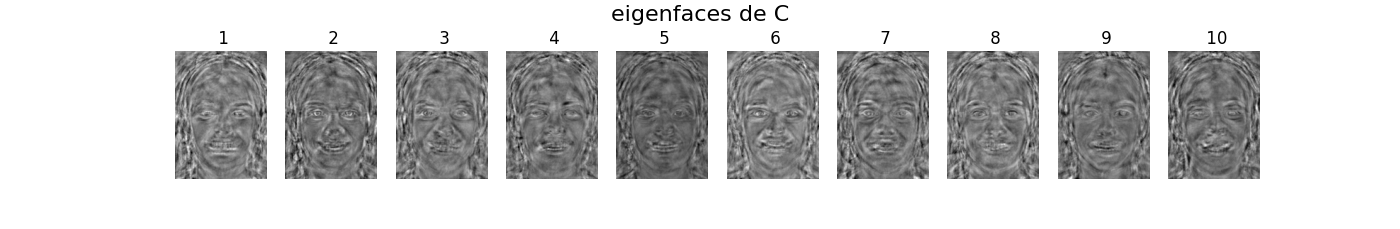
\includegraphics[width=1\textwidth]{img/MAIN_5.png}
                  \caption{Eigenfaces menos relevantes de cada matriz}
                  \label{fig:exemplo}
            \end{figure}

\end{frame}

\begin{frame}[c]{Eigenfaces}
\framesubtitle{Reconhecimento facial}

         Para reconhecer um rosto novo, é necessário projetar a imagem desse rosto nas eigenfaces para obter os coeficientes de projeção. Seja $\boldsymbol{z}$ o vetor de coeficientes de projeção de uma imagem de teste. Podemos calcular $\boldsymbol{z}$ da seguinte maneira:
 
            $$
            \boldsymbol{z} = \boldsymbol{U}^{T}(\boldsymbol{x_{teste}} - \boldsymbol{F_\mu})
            $$


            onde $\boldsymbol{x_{teste}}$ é o vetor de pixels da imagem de teste.

\end{frame}


\begin{frame}[c]{Discussão dos Resultados}
\framesubtitle{Reconstrução de Imagens}

    Suponha que queremos reconstruir a seguinte imagem:

        \begin{figure}[H]
                  \centering
                  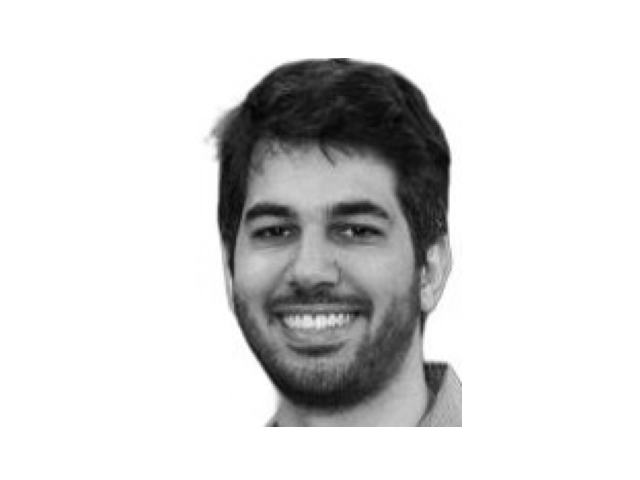
\includegraphics[width=0.5\textwidth]{img/MAIN_6.png}
                  \caption{Imagem a ser reconstruída}
                  \label{fig:exemplo}
        \end{figure}
\end{frame}

\begin{frame}[c]{Discussão dos Resultados}
\framesubtitle{Reconstrução de Imagens}

            \begin{figure}[H]
                  \centering
                  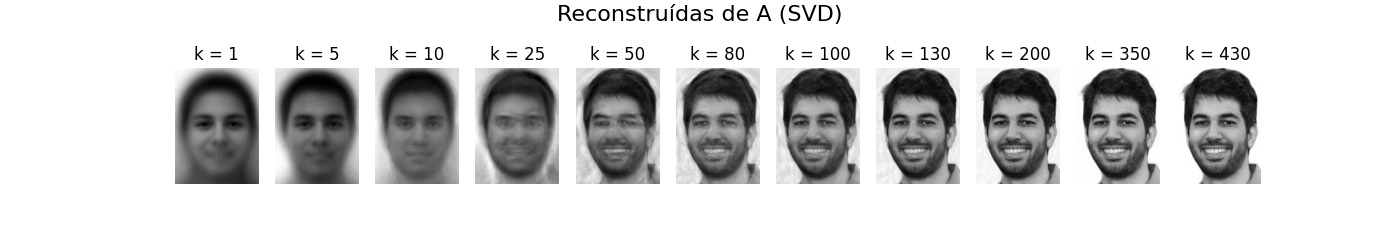
\includegraphics[width=1\textwidth]{img/reconstrucao_a.jpeg}
                  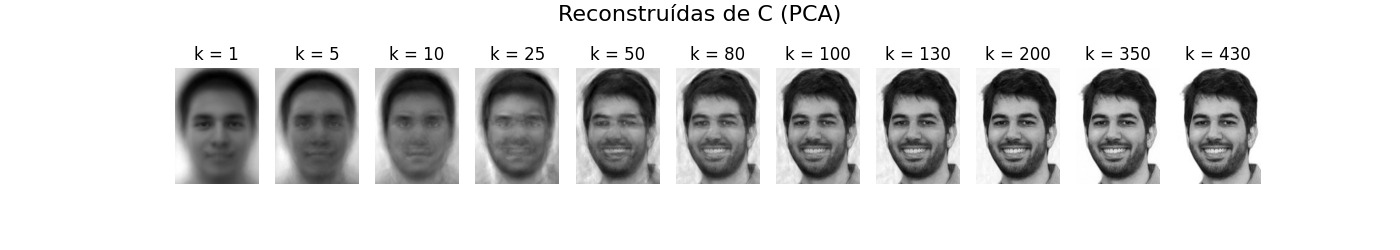
\includegraphics[width=1\textwidth]{img/reconstrucao_c.jpeg}
                  \caption{Imagem reconstruída}
                  \label{fig:exemplo}
        \end{figure}

\end{frame}

\begin{frame}[c]{Discussão dos Resultados}
\framesubtitle{Relevância das eigenfaces}

    \hfill
    \begin{figure}[H]
              \begin{subfigure}{0.4\textwidth}
                \centering
                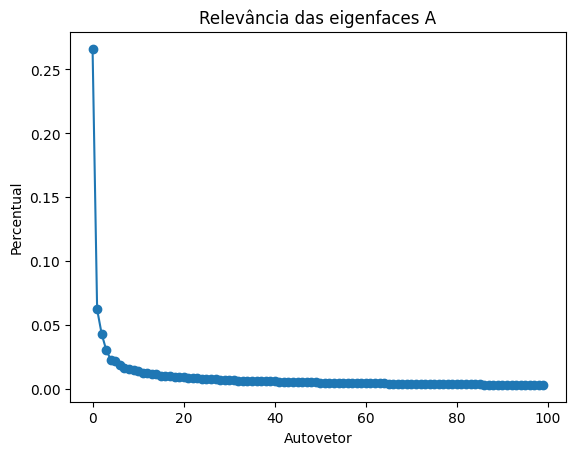
\includegraphics[width=\textwidth]{img/MAIN_10.png}
                \label{fig:imagem1}
              \end{subfigure}
              \hfill
              \begin{subfigure}{0.4\textwidth}
                \centering
                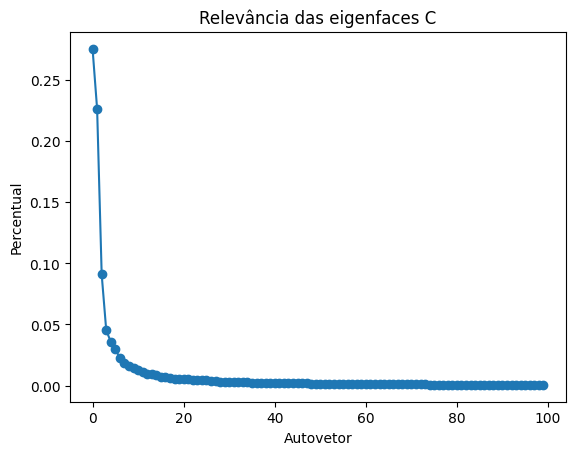
\includegraphics[width=\textwidth]{img/MAIN_11.png}
                \label{fig:imagem2}
              \end{subfigure}
              \caption{Relevância das Eigenfaces de cada matriz}
        \end{figure}
    \hfill

\end{frame}

\begin{frame}[c]{Discussão dos Resultados}
\framesubtitle{Custo Computacional}

    \begin{figure}[H]
                  \centering
                  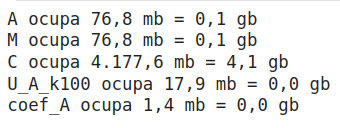
\includegraphics[width=0.5\textwidth]{img/memoria_ocupada.png}
                  \caption{Memória ocupada por cada matriz}
                  \label{fig:exemplo}
        \end{figure}

\end{frame}

\begin{frame}[c]
\frametitle{~}
    
    \begin{center}
        {\Huge Obrigado!}
    \end{center}
    
\end{frame}

\end{document} 
